%% Los cap'itulos inician con \chapter{T'itulo}, estos aparecen numerados y
%% se incluyen en el 'indice general.
%%
%% Recuerda que aqu'i ya puedes escribir acentos como: 'a, 'e, 'i, etc.
%% La letra n con tilde es: 'n.


\chapter{Introducción}

A lo largo de la historia de la agricultura, el hombre ha desarrollado el mejoramiento vegetal (o fitomejoramiento) en forma sistemática y lo ha convertido en un instrumento esencial para la mejora de la producción agrícola en términos de cantidad, calidad y diversidad.  

La humanidad depende, directa o indirectamente, de las plantas. Para la alimentación, ya que todos sus alimentos son vegetales o se derivan de éstos por ejemplo: carne, huevos y productos lácteos. De las plantas se deriva también la mayoría de las fibras textiles, fármacos, combustibles, lubricantes y materiales de construcción.

El fitomejoramiento, en un sentido amplio, es el arte y la ciencia de alterar o modificar la herencia de las plantas para obtener cultivares (variedades o híbridos) mejorados genéticamente, adaptados a condiciones específicas, de mayores rendimientos económicos y de mejor calidad que las variedades nativas o criollas \citep{Allard67}. En otras palabras, el fitomejoramiento busca crear plantas cuyo patrimonio hereditario esté de acuerdo con las condiciones, necesidades y recursos de los productores rurales, de la industria y de los consumidores, o sea de todos aquellos que producen, transforman y consumen productos vegetales. 

Las variedades mejoradas son el resultado del trabajo de desarrollo genético llevado a cabo en los programas de fitomejoramiento, los cuales se extienden a lo largo de varios años y requieren cuantiosas inversiones. La vigencia comercial de las variedades puede extenderse durante varias décadas, por lo que su elección es crítica para que el productor evite pérdidas económicas por malas campañas y el suministro al mercado sea constante. 

Generalmente, en etapas tempranas de estos programas existen un gran número de genotipos experimentales con pocos antecedentes de evaluación; mientras que en etapas posteriores  se trabaja con pocos genotipos altamente selectos. 

La utilización adecuada de procedimientos de análisis de datos agronómicos y ambientales es una condición inherente al desarrollo actual y futuro de investigaciones orientadas a mejorar los cultivos en forma económica y ambientalmente sustentable. En etapas avanzadas de los programas de mejoramiento, los ensayos multiambientales (EMA) que comprenden experimentos en múltiples ambientes son herramientas fundamentales para incrementar la productividad y rentabilidad de los cultivos. Estos son frecuentes en investigaciones agricolas de comparación de rendimiento, ya que constituyen una de las principales estrategias de identificación de genotipos vegetales superiores y de ambientes en los cuales estos se expresan de manera diferencial.

Debido a que las regiones de producción de los principales cultivos cubren áreas ecológicas muy extensas, se observan variaciones en las condiciones climáticas y de suelo. Por lo tanto, la aparición de la interacción genotipo ambiente (IGA) es inevitable, provocando respuestas altamente variables en los diferentes ambientes (Crossa et al., 1990; Cruz Medina, 1992; Kang y Magari, 1996). La IGA es considerada casi unánimemente por los fitomejoradores como el principal factor que limita la respuesta a la selección y, en general, la eficiencia de los programas de mejoramiento. 

Los investigadores agrícolas han sido conscientes de las diversas implicaciones de IGA en los programas de mejoramiento (Mooers, 1921; Yates y Cochran, 1938). Por ejemplo, la IGA tiene un impacto negativo en la heredabilidad, cuanto menor sea la heredabilidad de un caracter, mayor será la dificultad para mejorar ese caracter mediante la selección.
Por lo tanto, información sobre la estructura y la naturaleza de la IGA es particularmente útil para los mejoradores porque puede ayudar a determinar si necesitan desarrollar cultivares para todos los ambientes de interés o si deberían desarrollar cultivares específicos para ambientes específicos (Bridges, 1989). Gauch y Zobel (1996) explicaron la importancia de IGA como: “Si no hubiera interacción, una sola variedad de trigo (\emph{Triticum aestivum} L.) o maíz (\emph{Zea mays} L.) o cualquier otro cultivo rendiria al máximo en todo el mundo, y además la prueba de variedades deberia realizarse en un sólo lugar para proporcionar resultados universales. No habría ruido, los resultados experimentales serían exactos, identificando la mejor variedad sin error, y no habría necesidad de replicación. Entonces, una réplica en un lugar identificaría la mejor variedad de trigo que florece en todo el mundo ".

Peto (1982) ha distinguido las interacciones cuantitativas, llamada tambien sin cambio de rango (NCOI), o \emph{no crossover}, de las interacciones cualitativas, denominada tambien con
cambio de rango (COI) o \emph{crossover}(Cornelius et al., 1996). Cuando dos genotipos X e Y tienen una respuesta diferencial en dos ambientes diferentes, pero su ordenación permanece sin cambios se dice que la IGA es \emph{no crossover} (Figura \ref{fig:fig11}(A)). Sin embargo, es de tipo \emph{crossover} cuando hay cambios en el orden de los genotipos (Figura  \ref{fig:fig11}(B)). Cuando los genotipos responden de manera similar en ambos ambientes (Figura \ref{fig:fig11}(C)) no hay IGA. 


\begin{figure}[h]
\begin{center}
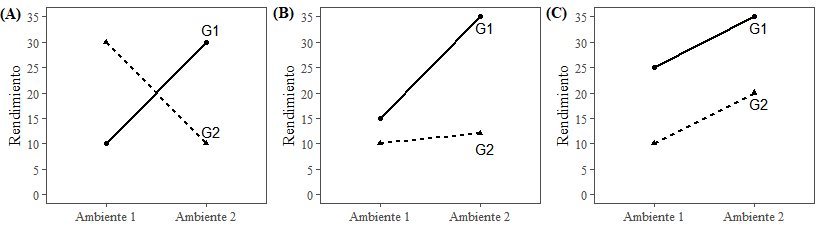
\includegraphics[width=14cm]{./Graficos/interac}
\end{center}
\caption{Representación gráfica de tipos de IGA: (A)IGA no crossover, (B) IGA crossover y (C) no IGA}
\label{fig:fig11}
\end{figure}


Distintos conceptos como regiones ecológicas, ecotipos, mega-ambientes, adaptaciones de germoplasma tanto en sentido amplio (a través de los ambientes) como específico (para cada ambiente o grupos de ambiente particular) (Kang et al., 2004) se pueden analizar a partir de la interacción genotipo-ambiente (Yan y Hunt, 2001).


Un análisis adecuado de la información de los EMA es indispensable para que el programa de mejoramiento de los cultivos sea eficaz. El rendimiento medio en los ambientes es un indicador suficiente del rendimiento genotípico solo en ausencia de IGA (Yan y Kang, 2003). Sin embargo, la aparición de IGA es inevitable y no basta con la comparación de las medias de los genotipos, sino que se debe recurrir a una metodología estadística más aporopiada. La metodología estadística más difundida para analizar los datos provenientes de EMA se basa en modificaciones de los modelos de regresión, análisis de variancia (\emph{Analysis of Variance}, ANOVA) y técnicas de análisis multivariado. 


Particularmente, para el estudio de la interacción y los análisis que de ella se derivan, dos modelos multiplicativos han aumentado su popularidad entre los fitomejoradores como una herramienta de análisis gráfico: el modelo de los efectos principales aditivos y interacción multiplicativa (\emph{Additive Main effects and Multiplicative Interaction}, AMMI) (Kempton 1984, Gauch, 1988), y el de regresión por sitio (\emph{Site Regression model}, SREG) (Cornelius et al., 1996; Crossa y Cornelius, 1997 y 2002).  Estos modelos combinan un ANOVA con la descomposición de valores singulares (DVS) o el análisis de componentes principales (ACP) sobre la matriz residual de ANOVA. En SREG, el ANOVA se realiza sobre el efecto principal de A mientras que en AMMI se considera el efecto de G y A. Mientras que a través del modelo AMMI se obtiene el gráfico biplot \emph{Genotipe-Environment} (GE) el cual es usado para explorar patrones puramente atribuibles a los efectos GE, para el modelo SREG, Yan y Hunt (2002), presentaron la técnica GGE biplot usado para explorar simultáneamente patrones de variación en la suma G+GE.

Una limitación importante de la mayoría de las propuestas de análisis provenientes de EMA es que requieren que el conjunto de datos este completo. Aunque los EMA están diseñados para que todos los genotipos se evalúen en todos los ambientes,  las tablas de datos genotipo x ambiente completas son poco frecuentes (no todos los genotipos se encuentran en todos los ambientes). Esto ocurre, por ejemplo, debido a errores de medición o causas naturales como, por ejemplo, la destrucción de plantas por animales, inundaciones o durante la cosecha, la incorporación de nuevos genotipos y a que otros se descartan por su pobre desempeño (Hill y Rosemberg, 1985). En estos casos, entre las posibles soluciones para tratar con una tabla de datos incompleta es (i) el uso de un subconjunto completo de datos, eliminando aquellos genotipos que tienen valores faltantes (Ceccarelli et al., 2007, Yan et al., 2011), (ii) completar datos faltantes con la media ambiental, o (iii) imputación de datos faltantes con valores estimados utilizando, por ejemplo, un modelo multiplicativo (Kumar et al., 2012). 

En este contexto, el análisis de datos provenientes de EMA requiere metodología estadística sofisticada cuyas rutinas informáticas se encuentran disponibles en programas desarrollados por diferentes empresas. Esto genera el inconveniente de tener que disponer de todos los programas necesarios para los distintos análisis, atender los requerimientos de formatos de datos usados por cada uno, y comprender los diversos tipos de salidas en las que se ofrecen los resultados obtenidos. Además, algunos procedimientos, especialmente aquellas metodologías recientes, no se encuentran dispobibles, y los costos de las licencias de dichos programas resultan muy elevados. 


El software R se trata de un proyecto de software libre distribuido bajo los términos de la \emph{General Public Licence} (GNU), desarrollado por \emph{The R Foundation for Statistical Computing}. Surge como resultado de la implementación de uno de los lenguajes más utilizados en investigación por la comunidad estadística, el lenguaje S. Que un software sea libre quiere decir que sus usuarios son libres de usarlo, copiarlo, distribuirlo, editarlo y modificarlo según sus propias inquietudes (FSF 2019). A diferencia de los programas estadísticos utilizados frecuentemente, R es un lenguaje de programación y no dispone de una interfaz gráfica en la cual se utilizan menues para realizar los distintos análisis de interes, lo cual genera dificultad en su uso para aquellos que no se encuentran familiarizados con el uso de código computacional. Sin embargo, brinda mayores posibilidades en cuanto a la manipulación y análisis de los datos ya que le permite a los usuarios definir sus propias funciones y pesonalizar el tipo de análisis que desean realizar. Si bien la versión básica del programa dista mucho de ser amigable, R Studio permite contar con una interacción más fluida con el programa R actuando como una interfaz amigable entre el usuario.  RStudio es un entorno de desarrollo integrado (IDE) gratuito y de código abierto para R. 

R forma parte de un proyecto colaborativo ya que promueve el hecho de que los usuario creen funciones y las ponga al alcance de toda la comunidad, es decir que está en continuo desarrollo y actualización.  Sin embargo, como muchas veces no resulta sencillo reutilizar una función creada por algun usuario se ha introducido la posibilidad de crear paquetes (\emph{package}) o librerías. Estas son una colección de objetos creados y organizados siguiendo un protocolo fijo que garantiza un soporte mínimo para el usuario así como la ausencia de errores (de sintaxis) en la programación.

R cuenta con 14 paquetes básicos y 29 recomendados para su funcionamiento instalados automaticamente en él, como por ejemplo, \emph{base} o \emph{stats}. Dado que la comunidad de usuarios que programan en R ha ido creciendo notablemente en los últimos años y que muchos de ellos han ido proporcionando librerías, se cuenta con una gran cantidad de paquetes que extienden las funciones básicas de R. Entre ellos se encuentran, \emph{plyr}, \emph{lubridate}, \emph{reshape2} y \emph{stringr} para la manipulación de los datos; \emph{ggplot2} y \emph{rgl} para la visualización; \emph{knitr} y \emph{xtable} para la presentación de resultados; entre otros. La lista completa de los paquetes oficiales puede consultarse en CRAN\footnote{CRAN (Comprehensive R Archve Network) es el repositorio oficial de paquetes de R, el lugar donde se publican las nuevas versiones del programa, etc. Contiene la lista completa de paquetes oficiales. \url{https://cran.r-project.org/web/packages/available_packages_by_name.html}}, se contaba con más de 14.000 paquetes disponibles en CRAN hasta junio de 2019. Esta gran variedad de paquetes es una de las razones por las que R tiene tanto éxito: lo más probable es que alguien ya haya resuelto un problema en el que estás trabajando, y puedes beneficiarte de su trabajo descargando su paquete.

Además de los paquetes oficiales, existen otros que pueden instalarse desde repositorios como, por ejemplo, Github. Sin embargo, no es sencillo encontrar un paquete que puede ser útil para un determinado fin sino que se debe recurrir a varios de ellos para cumplir un determinado objetivo. 

La decisión de qué software de análisis estadístico utilizar no tiene una respuesta predeterminada: la elección dependerá de las necesidades de la investigación. Esto pues los lenguajes de programación son herramientas y el principal criterio para decidir el uso de uno u otro debe efectuarse en función de la particularidad de los objetivos y alcances de la investigación que se busque desarrollar.

Frecuentemente, los mejoradores utilizan programas que tienen una interfaz gráfica para realizar los análisis estadísticos deseados y no tienen un manejo fluido de un lenguaje de programación. En el año 2012 se creó el paquete \emph{Shiny} de R que permite desarrollar aplicaciones Web utilizando R, acercando la potencia de R a todo tipo de usuarios.


El objetivo del presente trabajo fue: (i) crear un paquete de R que incluya las funciones que permitan analizar los datos provenientes de EMA, incluyendo además metodología recientemente publicada que no se encuentra disponible en R; (ii) crear una interfaz gráfica, entre R y el usuario, mediante Shiny con el fin de poder realizar los análisis disponibles en el paquete creado sin necesidad de utilizar el lenguaje de programación.



Elousa, Paula. 2009. “¿EXISTE VIDA MÁS ALLÁ DEL SPSS? DESCUBRE R.” Revista Psicothema 21 (4): 652–55. http://www.psicothema.com/psicothema.asp?id=3686.

FSF. 2019. “¿Qué Es El Software Libre?” Free Software Foundation. https://www.fsf.org/es/recursos/que-es-el-software-libre.